This chapter provides detailed specifications of the system under development.

% \section{Functional Requirements}

% This section describes each function/feature provided by our system. These functions are logically grouped into modules based on their purpose/users/mode of operations etc (as per our system). A functional hierarchy may look like:
% \begin{outline}
%   \1 Module 1:
%   \2 Function 1:
%   \2 Function 2:
%   \3 Sub Function 1
%   \3 Sub Function 2
%   \1 Module 2:
%   \2 Function 1:
%   \2 Function 2:
%   \1 .........
% \end{outline}

% % --- The above is to be modified as per your project, e.g. a flat list if your system has limited functional requirements.

% \section{Non-functional Requirements}

% This sections mentions the specific non-functional requirements of our system. These generally address performance, scalability, safety, availability, deployment etc.

\section{External Interfaces}

% We expect every project to have at least of the following subsections. This section must be aligned with your project deliverables. Please consult with your project supervisor regarding which of the following section(s) you should include in your report

\subsection{User Interfaces}
The User interface for this project will include a simulation interface built on Netlogo as one of the final deliverables. The user will be able to simulate the growth and optimization of Mycelium networks. This simulation interface will support parameters such as position of food nodes, and starting point of mycelium colonization, among other variables.

\subsection{Application Program Interface (API)}
Images of natural systems might represent patterns of network-like structure, which might reveal vital data regarding the topological properties of the underlying subject. However, the image itself doesn't mechanically offer a proper definition of a network in terms of sets of nodes and edges. Instead, this information ought to be fittingly extracted from the raw image data. Our system will make use of the following libraries for graph acquisition and its analysis; especially in our case where mycelium networks’ data collection relies on images where graph extraction requires domain-specific solutions:
\begin{itemize}
    \item NEFI 2.0: A tool that extracts graphs from images of networks originating in various domains. NEFI provides a completely unique platform permitting practitioners to simply extract graphs from pictures by combining basic tools from image processing, computer vision and graph theory. We anticipate NEFI to enable time-efficient collection of large datasets. It is a flexible toolbox based on a combination of standard image-processing routines. Depending on the characteristics of the input image and therefore the elected pipeline, the standard of the ensuing graph could vary. NEFI's accuracy reflects how closely the computed graph resembles the originally portrayed input network. Thus, once performing segmentation as necessary step in network extraction, NEFI inherits the strengths and the weaknesses of its algorithms.
    \item MathWorks’ Image Processing (IPT) and Computer Vision Toolboxes (CVT): IPT provides a comprehensive set of reference-standard algorithmic programs and advancement apps for image processing, analysis, visualization, and algorithm development. We will perform image phaseation, image enhancement, noise reduction, geometric transformations, image registration, and 3D image processing. Image process tool case apps allow you to automatize common image processing workflows. We will interactively segment image knowledge, compare image registration techniques, and batch-process giant data sets.
    
    CVT provides algorithms, functions, and apps for planning and testing laptop vision, 3D vision, and video processing systems. We will perform object detection and tracking, further as feature detection, extraction, and matching. The tool case provides object detection and segmentation algorithms for analyzing pictures that are overlarge to suit into memory.
    \item NetLogo Py Extension: The general workflow of this extension is to run py:setup py:python to initialize the Python session that NetLogo will talk to, and then use py:run, py:runresult, and py:set to interact with that Python session.
\end{itemize}

\subsection{Hardware/Communication Interfaces}
This project will include a digital image processing phase where we will use images of Mycelium growth taken at timed intervals, to extract the apparent network from these images. This extraction process is going to be supported using \href{http://nefi.mpi-inf.mpg.de}{NEFI 2.0} which is an open-source python tool that allows for extraction of graphical data from images and outputs it in terms of a weighted undirected planar graph. This graphical data will then be used for analysis, and eventually to form the basis for the algorithm to simulate the growth of Mycelium networks.

%\section{Use Cases}
%This section presents detailed use cases of our system.

\section{Datasets}
Our project aims to use datasets representing Mycelium networks in terms of graphs, using an adjacency list or matrix representation. So far we haven't come across an open-source dataset which meets our requirement, however in their paper "Network Organisation of Mycelial Fungi" Fricker and et al. \cite{networkmyc} stored their network data in the form of adjacency matrices which we are hoping to procure from them if feasible (the data remained unpublished). Concurrently, we are also searching for datasets in the form of images of culture growth on agar plates with timed intervals. We can extract such data using NEFI 2.0. 

\section{System Diagram}
This diagram gives a high-level view of the different components of our system and the interactions between them. Each component and the particular tools/technologies/libraries used to build it are described.

\begin{figure}[h!]
    \centering
    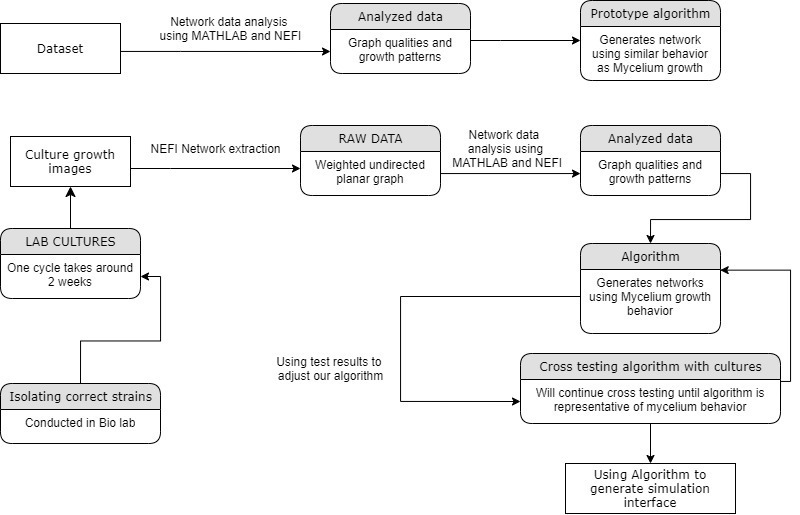
\includegraphics[scale=0.5]{Images/system_diag.png}
    \caption{System Diagram}
    \label{fig:sys_diag}
\end{figure}